\section{Execution phase}



\subsection*{Step 1}
\begin{figure}[!htb]
	\centering
	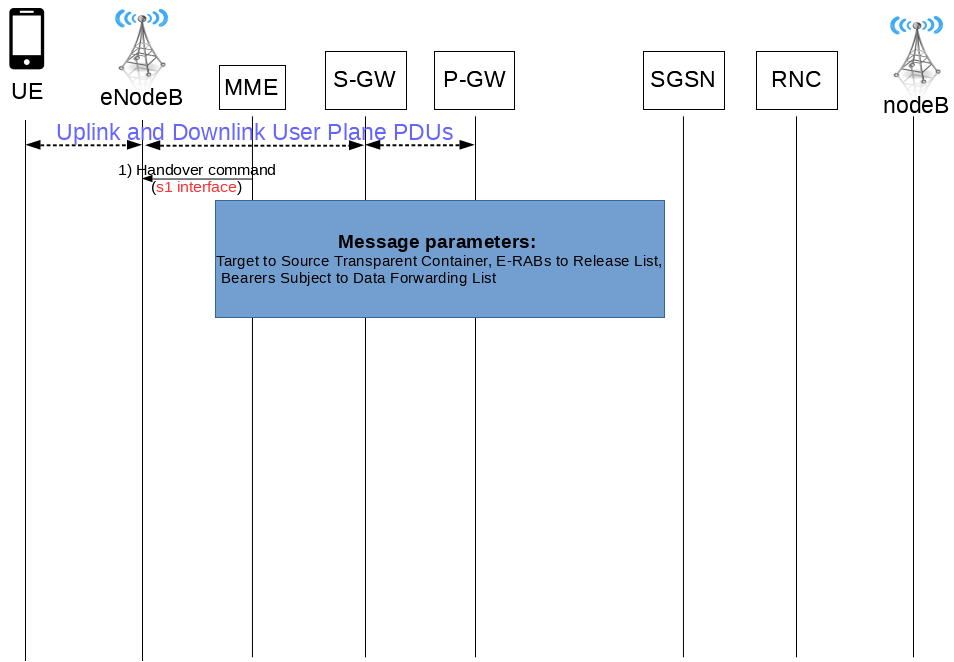
\includegraphics[width=0.9\linewidth]{img/execution-1.png}
	\label{fig:exec-1}
\end{figure}
The source MME completes the preparation phase by sending to the source eNodeB
the \emph{Handover command} message through the interface S1. The message
contains the following parameters:
\begin{itemize}
    \item Target to Source Transparent Container
    \item E-RABs to Release List
    \item Bearers Subject to Data Forwarding List: if ``Direct
    Forwarding'' applies it is the list of ``Address(es) and TEID(s) for user
    traffic data forwarding'' received from the target SGSN during step 5
    of the preparation phase (addresses and GTP-U tunnel endpoint parameters to
    the Target RNC or to the target SGSN if direct tunnel is used), otherwise
    if ``Indirect Forwarding'' applies it contains the parameters received in
    step 6a (S-GW addresses)
\end{itemize}



\clearpage
\subsection*{Step 2}
\begin{figure}[!htb]
	\centering
	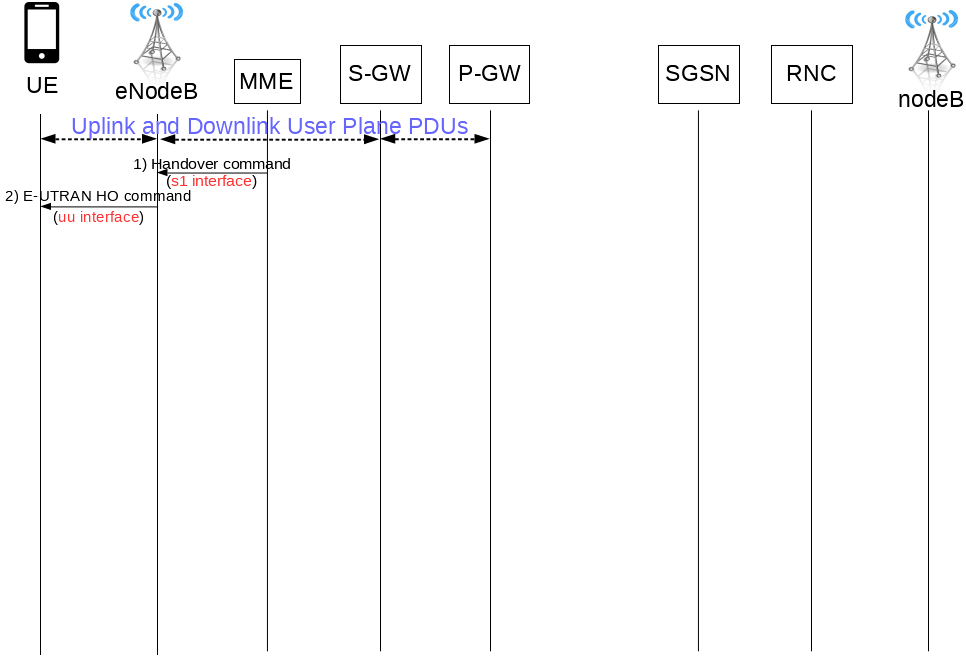
\includegraphics[width=0.9\linewidth]{img/execution-2.png}
	\label{fig:exec-2}
\end{figure}

The source eNodeB initiates data forwarding for bearers specified in the
``Bearers Subject to Data Forwarding List'' of the message received from the MME.

After that, the eNodeB sends the E-UTRAN command \emph{HO} to the UE for telling
it to handover to the target access network. This message includes a transparent
container which contains the radio parameters that the RNC has set-up during the
preparation phase. The message is sent through the DCCH logical channel, which
maps to the DL-SCH transport channel, which maps to PDSCH physical channel \cite{channels}.

After the reception of the HO command the UE has to associate its bearer IDs to
the respective RABs according to the relation with the NSAPIs\footnote{NSAPI is
used to identify PDP contexts in the SGSN. A PDP context is a data structure
which contains subscriber's session information such as its IMSI and its IP
address} and has to suspend the uplink transmission of user data.



\subsection*{Step 3}
\begin{figure}[!htb]
	\centering
	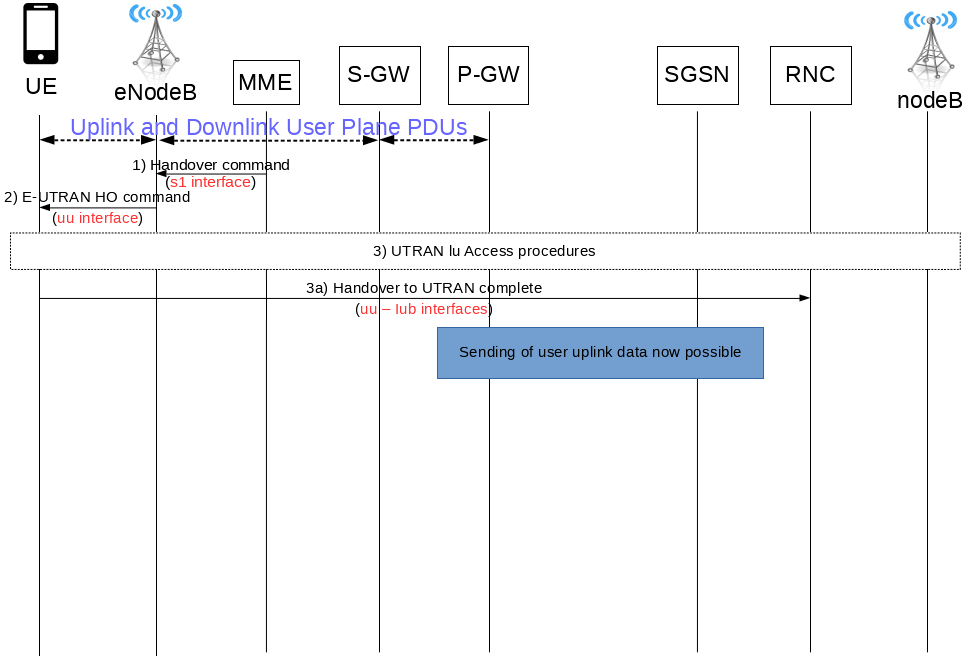
\includegraphics[width=0.9\linewidth]{img/execution-3.png}
	\label{fig:exec-3}
\end{figure}
The UE executes the handover to the target UTRAN according to the prameters
contained in the message received in step 2. At this point it can resume the user
data transfer only for those NSAPIs which have been associated to a RAB, namely
the NSAPIs for which there are radio resources allocated in the target RNC.




\subsection*{Step 4}
\begin{figure}[!htb]
	\centering
	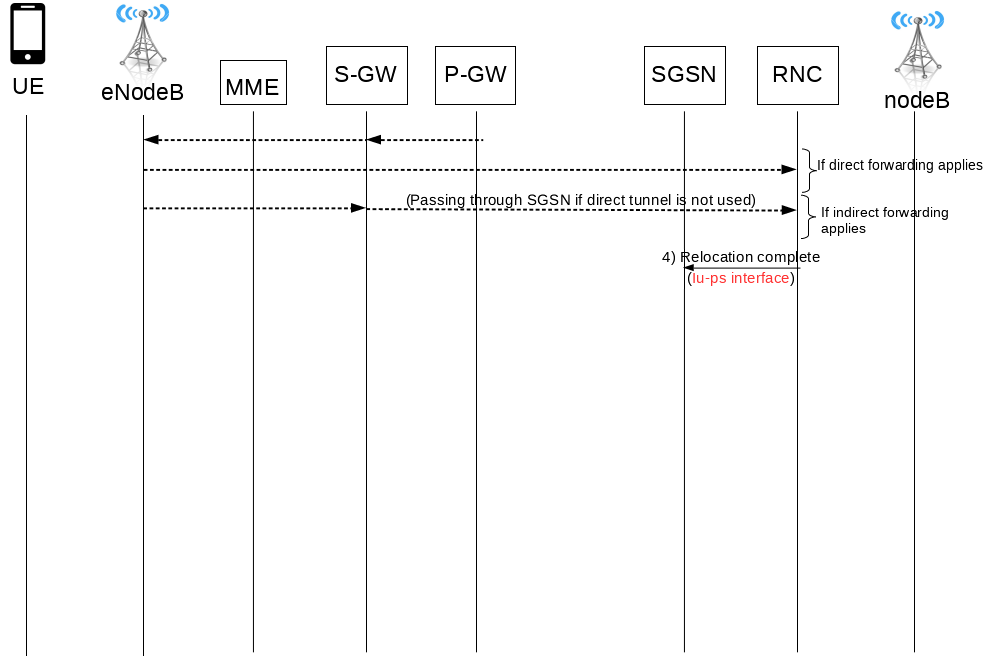
\includegraphics[width=0.9\linewidth]{img/execution-4.png}
	\label{fig:exec-4}
\end{figure}
After the RNC-ID and the S-RNTI\footnote{In UMTS the S-RNTI is the UE identifier which is allocated
by the RNC and it's unique within that RNC} are exchanged with the UE, the target
RNC sends the \emph{Relocation Complete} message to the target SGSN, indicating
therefore the completion of the relocation from the source E-UTRAN to the target
RNC. After receiving this message, the SGSN is ready for receiving data from
the target RNC.




\subsection*{Step 5}
\begin{figure}[!htb]
	\centering
	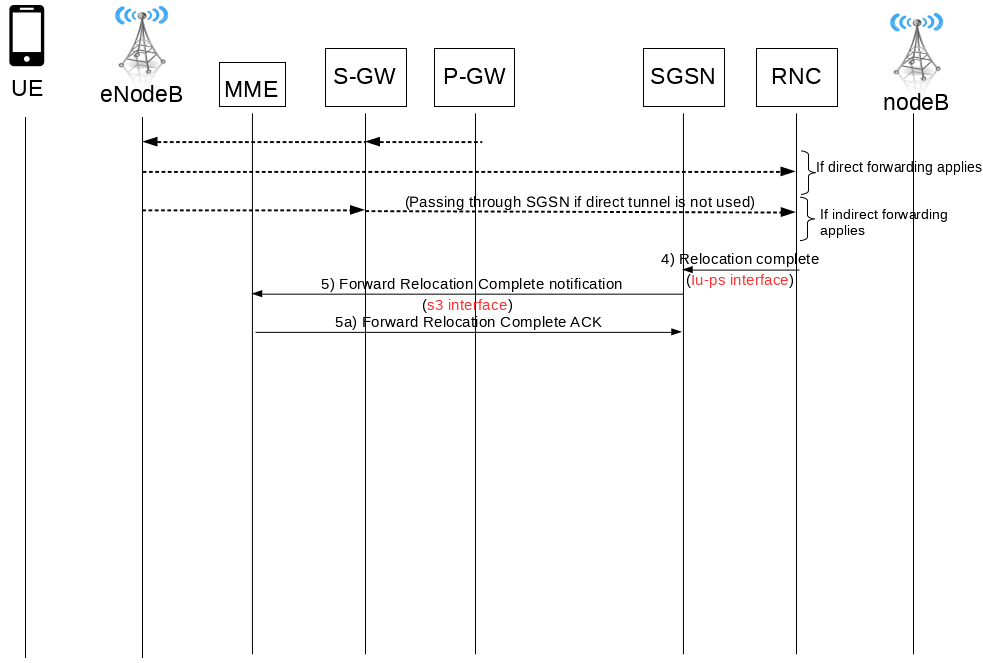
\includegraphics[width=0.9\linewidth]{img/execution-5.png}
	\label{fig:exec-5}
\end{figure}
The target SGSN informs the source MME that the UE has arrived to the target side
(UMTS network) by sending the Forward Relocation Complete Notification message.

When the MME receives the message it starts a timer and it releases all the bearers
that were not included in the Forward Relocation Request message sent in step 3
of the preparation phase by sending a Delete Bearer Command to the S-GW.

When the timer expires, if ISR Activated was not indicated in the message received
from the SGSN and Indirect Forwarding is used (and therefore the SGSN allocated
S-GW resources for it), the MME releases all the bearer resources of the UE by
sending Delete Indirect Data Forwarding Tunnel Request message to the S-GW used
for indirect forwarding (see step 9).



\subsection*{Step 6}
\begin{figure}[!htb]
	\centering
	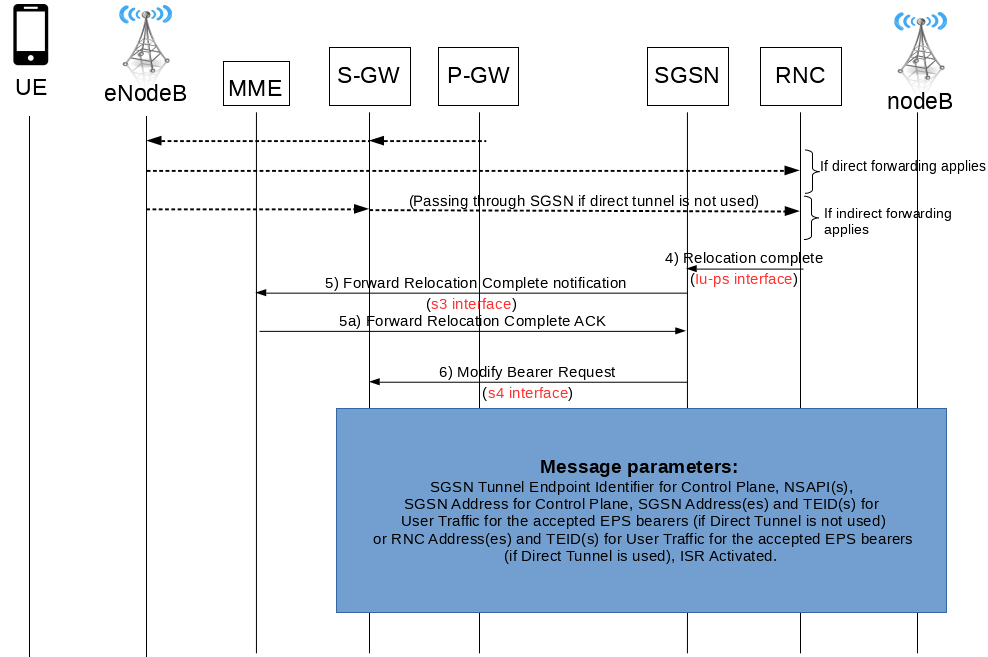
\includegraphics[width=0.9\linewidth]{img/execution-6.png}
	\label{fig:exec-6}
\end{figure}
The SGSN informs the S-GW that now the SGSN is responsible for all the EPS Bearer
contexts that the UE has established by sending to it a Modify Bearer request per
each PDN connection. The message contains the following parameters:
\begin{itemize}
	\item SGSN address and Tunnel Endpoint Identifier for Control Plane
	\item NSAPI(s)
	\item SGSN Address(es) and TEID(s) for User Traffic for the accepted EPS bearers
	(if Direct Tunnel is not used)
	\item RNC Address(es) and TEID(s) for User Traffic for the accepted EPS bearers
	(if Direct Tunnel is used)
	\item RAT type
	\item ISR Activated
	\item User location information (only if the SGSN supports location information
	change reporting)
\end{itemize}
??? The SGSN releases the non-accepted EPS Bearer contexts by triggering the Bearer Context deactivation
procedure. If the Serving GW receives a DL packet for a non-accepted bearer, the Serving GW drops the DL
packet and does not send a Downlink Data Notification to the SGSN. ???




\subsection*{Step 7}
\begin{figure}[!htb]
	\centering
	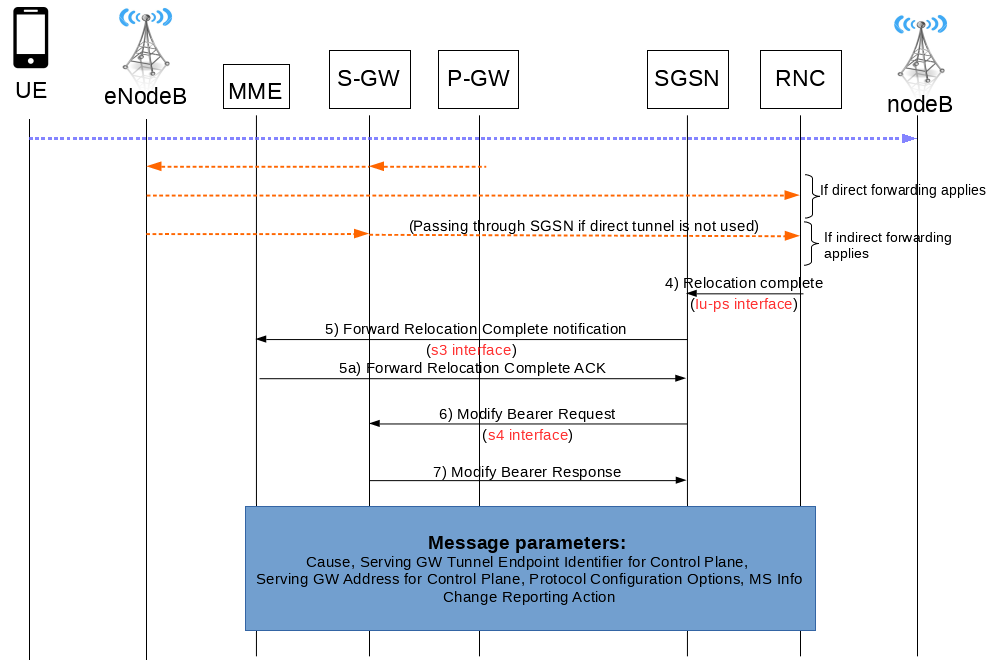
\includegraphics[width=0.9\linewidth]{img/execution-7.png}
	\label{fig:exec-7}
\end{figure}
The S-GW sends to the SGSN the Modify Bearer Response message for acknowledging
the user plane switch to the target SGSN.

After this step the user data path is finally established and it's shown in
figure \ref{fig:final-data-path}.

\begin{figure}[!htb]
	\centering
	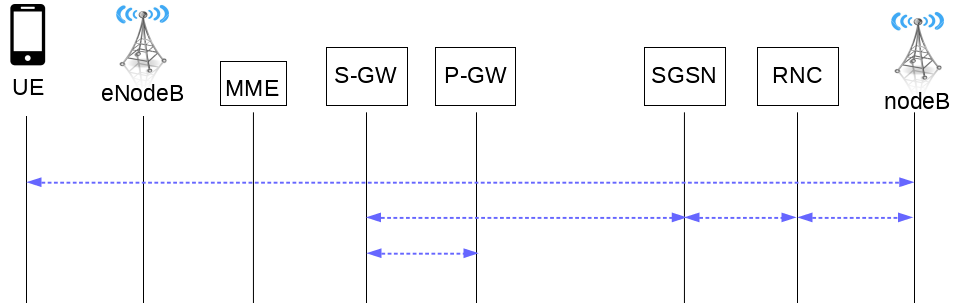
\includegraphics[width=0.9\linewidth]{img/final-data-path.png}
	\caption{The user data path after the step 7. In this case it is assumed that
	direct tunnel is not used, therefore the link between the RNC and the S-GW passes
	through the SGSN. If direct tunnel is instad used then the data go straight
	from the RNC to the S-GW.}
	\label{fig:final-data-path}
\end{figure}




\subsection*{Step 8}
When the UE recognises that its current Routing Area is not registered with the
network, or when the UE's TIN indicates "GUTI", the UE initiates a Routing Area
Update procedure with the SGSN. This procedure is the UMTS equivalent of the
Tracking Area Update procedure in LTE and it's described in reference
\cite{routing-area-update}.




\subsection*{Step 9}
If indirect forwarding was used then when the timer started by the MME at step 5
expires the MME sends a Delete Indirect Data Forwarding Tunnel Request message
to the S-GW for releasing the temporary resources used for indirect forwarding.
\begin{figure}[!htb]
	\centering
	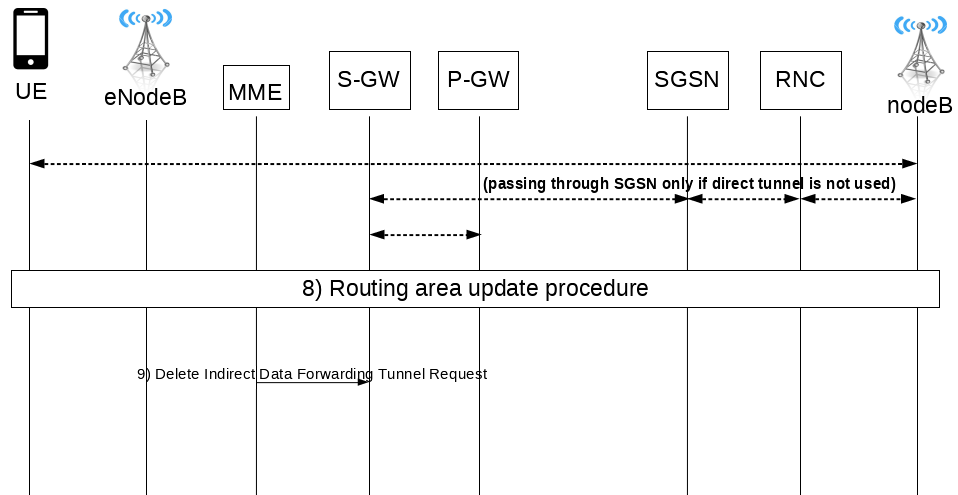
\includegraphics[width=0.9\linewidth]{img/execution-9.png}
	\label{fig:exec-9}
\end{figure}
